\documentclass[10pt,a4paper,notumble]{leaflet}
\usepackage[T1]{fontenc}
\usepackage[ngerman]{babel}
\usepackage[utf8]{inputenc}
\usepackage{color,flowfram,graphicx}
	\graphicspath{{./bilder/}}
\usepackage{wrapfig,rotating}
\usepackage{multirow,multicol,array,mathpazo}
\usepackage{titlesec}
\usepackage{framed,libertine}
\usepackage[usenames,dvipsnames,svgnames]{xcolor}
\usepackage{rotating}

\usepackage{setspace,fontawesome} %fb and youtube icon
\usepackage[colorlinks=true, urlcolor=black]{hyperref}
\urlstyle{same}

\definecolor{ffyellow}{RGB}{255,180,0}
\definecolor{ffred}{RGB}{220,0,103}
\definecolor{ffblue}{RGB}{0,158,224}
\definecolor{ffgrey}{RGB}{51,51,51}

\titleformat*{\section}{\Large\color{ffred}}



%FONT Change
%\renewcommand{\familydefault}{cmss} 

% To draw a horizontal Line
\newcommand{\sectionline}{
 \nointerlineskip \vspace{\baselineskip}
 \hspace{\fill}\rule{0.8\linewidth}{.7pt}\hspace{\fill}
 \par\nointerlineskip \vspace{\baselineskip}
}

% Add graphics to bottom of the first page
\AddToBackground{2}{
\includegraphics[width=9.9cm]{aufkleber_hh.pdf}}

% Make a border along the top of each page
\setmargins{15mm}{15mm}{7mm}{7mm}
\vtwotonetop{1cm}{0.6\paperwidth}{ffyellow}{topleft}{0.4\paperwidth}{ffyellow}{topright}
\vtwotonebottom[1,6]{1cm}{0.6\paperwidth}{ffyellow}{bottomleft}{0.4\paperwidth}{ffyellow}{bottomright}

\pagestyle{empty}



\begin{document}

% \begin{titlepage}
% \title{Teilt Eure WLANs!}
% \date{}
% \end{titlepage}

% \maketitle

\begin{center}
{\fontsize{70}{90}\selectfont \faWifi}
\end{center}
\begin{center}
{\fontsize{30}{40}\selectfont Teilt\ Eure WLANs!}
\end{center}

\vfill

{\fontsize{16}{18}\selectfont Tausende weimarer Schüler:innen befinden sich im Fernunterricht. Dank Corona ist die Digitalisierung quasi über Nacht auch in den Schulen angekommen. Doch nicht alle Schüler:innen haben zu Hause einen Internetzugang. Mit Freifunk kannst Du helfen und Deinen Internetzugang einfach und sicher teilen.\par}

\vspace{4em}

\begin{center}

\includegraphics[width=80mm]{aufkleber_we.pdf}
\end{center}


\thispagestyle{empty}
\newpage

\section{Was ist Freifunk?}
Freifunk ist eine nichtkommerzielle Initiative für freie Funk\-netzwerke. Wir bauen ein Gemeinschaftsnetz und stellen anderen unsere Internetzugänge zur Verfügung. In diesem Flyer erfährst Du wie Du mitmachen kannst.

Du brauchst keine besonderen technischen Kenntnisse, um Teil des Netzes zu werden. Es genügt, 1. ein passendes Gerät -- einen herkömmlichen WLAN-Router, den sog. Freifunk-Knoten -- zu kaufen, 2. die Freifunk-Firmware nach Anleitung aufzuspielen, 3. den Knoten einzurichten und 4. anzuschließen.

% Alternativ kannst Du bei TODO ein fertig eingerichtetes Gerät abholen, das nur noch angeschlossen werden muss.

\section{1. Gerät kaufen}
Je nach Geldbeutel und Installationsort eignen sich verschiedene Geräte. Wir empfehlen an dieser Stelle zwei Geräte, die leicht eingerichtet werden können: den \textbf{Netgear R6120} (ca. 40€) und den \textbf{Gl.iNet GL-B1300} (ca. 70€).

Grundsätzlich sind alle Geräte geeignet, die unter \href{https://www.weimarnetz.de/router}{https://www.weimarnetz.de/router} aufgeführt werden. Manche der dort aufgeführten Geräte gibt es in verschiedenen Hardware-Revisionen, bitte achtet beim Kauf darauf. Nicht immer werden alle Revisionen von uns unterstützt.

Sobald ein passendes Gerät beschafft wurde, kann die Firmware aufgespielt werden.


\newpage


\section{2. Firmware aufspielen}

\paragraph{Netgear R6120}
\begin{enumerate}
 \item Lade zunächst die Erstinstallations-Firmware für Dein Gerät herunter: \href{https://hamburg.freifunk.net/firmware}{https://hamburg.freifunk.net/firmware}
 \item Schließe den Router ans Stromnetz an. Warte bis die Power- und die WiFi-LED durchgehend eingeschaltet sind. Verbinde jetzt den \textit{LAN-Port 2} mit dem Netzwerkanschluss des Computers.
 \item Öffne in einem Browserfenster die Adresse \textit{http://routerlogin.net} bzw. \textit{http://192.168.2.2}
 \item Klicke links oben auf \textit{Erweitert} und dann im Reiter \textit{Administration} auf \textit{Firmwareupdate}.
 \item Wähle die Freifunk-Firmware aus und klicke anschließend auf \textit{hochladen} und auf \textit{OK}.
 \item Nun warte etwa drei Minuten bis das Upgrade durchgelaufen ist. Danach kann der Knoten eingerichtet werden.
\end{enumerate}


\paragraph{Gl.iNet GL-B1300}
\begin{enumerate}
 \item Lade zunächst die Firmware für Dein Gerät herunter: \href{https://hamburg.freifunk.net/firmware}{https://hamburg.freifunk.net/firmware}
 \item Schließe den Router ans Stromnetz an. Verbinde dann den \textit{mittleren LAN-Port} mit dem Netzwerkanschluss des Computers.
 \item Öffne in einem Browserfenster die Adresse \textit{http://192.168.8.1}
 \item Wähle nun eine Sprache und vergebe ein Passwort. Klicke danach links auf \textit{Aktualisierung} und dann auf den Reiter \textit{lokales Upgrade}.
 \item Wähle die Freifunk-Firmware aus, \textbf{deaktiviere} \textit{Einstellung behalten} und klicke anschließend auf \textit{Installieren}.
 \item Nun warte etwa drei Minuten bis das Upgrade durchgelaufen ist. Danach kann der Knoten eingerichtet werden.
\end{enumerate}


\newpage

\section{3. Knoten einrichten}
%Bilder unter https://hamburg.freifunk.net/anleitung/router-einrichten
Nach kurzer Wartezeit ist nun die neue Konfigurationsoberfläche unter http://192.168.1.1 erreichbar.

\begin{enumerate}
 \item Gib Deinem Knoten einen Namen und klicke auf \textit{Fertig}.
 \item Klicke jetzt auf den angezeigten Link. Dann wird automatisch das Knotenformular geöffnet und ausgefüllt. Wenn Du in diesem Formular die Geo-Koordinaten Deines Routers einträgst, ist er auf der Knotenkarte zu sehen. So können alle feststellen, wo überall Freifunk verfügbar ist. Diese Angabe ist freiwillig, aber empfohlen. Bitte gib auch einen Namen und eine gültige E-Mail-Adresse an, unter der Freifunk Dich bezüglich Deines Routers kontaktieren kann.
 \item Klicke auf \textit{Knoten anmelden} und notiere den \textit{Token}.
\end{enumerate}
Damit ist die Registrierung abgeschlossen und Du kannst Deinen Freifunk-Router nun in Betrieb nehmen.

\section{4. Knoten anschließen}
Verbinde die \textit{WAN-Buchse} des Freifunk-Knotens mit einer freien Buchse Deines Internet-Routers. Nach wenigen Minuten sollte der Router auf der Knotenkarte \mbox{https://map.hamburg.freifunk.net/} an der von dir angegebenen Position zu sehen sein.

Nun solltest Du ein neues, offenes WLAN mit der SSID \mbox{\textit{hamburg.freifunk.net}} sehen. Teste es am besten kurz und sage dann Deinen Nachbarn Bescheid!




\newpage
\section{Häufige Fragen}
\setlength{\parskip}{0.1em}
\paragraph{Wo stehen schon Freifunk-Router?} Eine Karte findest Du unter \href{https://map.hamburg.freifunk.net}{https://map.hamburg.freifunk.net}.

\paragraph{Was kostet Freifunk?}
Für die Nutzung fallen für Dich keine Kosten an. Die Infrastruktur wird ausschließlich über Spenden finanziert.

Falls Du selbst einen Freifunk-Zugang anbieten möchtest, benötigst Du einen eigenen Internetanschluss und einen passenden Router. Dieser kostet je nach Modell ab ca. 35€.  Neben den Stromkosten für das Betreiben des Routers fallen keine weitere Kosten an.

\paragraph{Wie weit reicht ein Freifunk-Knoten?} Freifunk nutzt ganz normales WLAN. Bei optimalen Bedingungen reicht das WLAN mehr als 100m weit. Jeder Gegenstand (Wand, Fenster, Baum, Mensch…) wirkt jedoch dämpfend auf das Signal. Praktisch reicht es oft zumindest bis in die Nachbarwohnung.

\paragraph{Ist das sicher?} Dein Freifunk-Knoten wird standardmäßig automatisch mit Updates versorgt. Außerdem kann man aus dem Freifunk-Netz nicht auf Dein privates Netz zugreifen.

Bei der Nutzung herrschen die gleichen Bedingungen wie in jedem anderen WLAN: Die Nutzer:innnen müssen verantwortlich damit umgehen. Das bedeutet u.a.: die eigenen Endgeräte (Handy, Laptop etc.) mit den üblichen Vorkehrungen vor Fremdzugriff zu schützen, Verschlüsselung \& https zu benutzen sowie regelmäßige Updates der Router und Endgeräte durchzuführen.

\paragraph{Wo kann ich weitere Informationen finden?} Auf unserer Webseite \href{https://hamburg.freifunk.net}{https://hamburg.freifunk.net} und im Freifunk-Wiki unter \href{https://wiki.freifunk.net/Hamburg}{https://wiki.freifunk.net/Hamburg}.

\newpage
\begin{center}
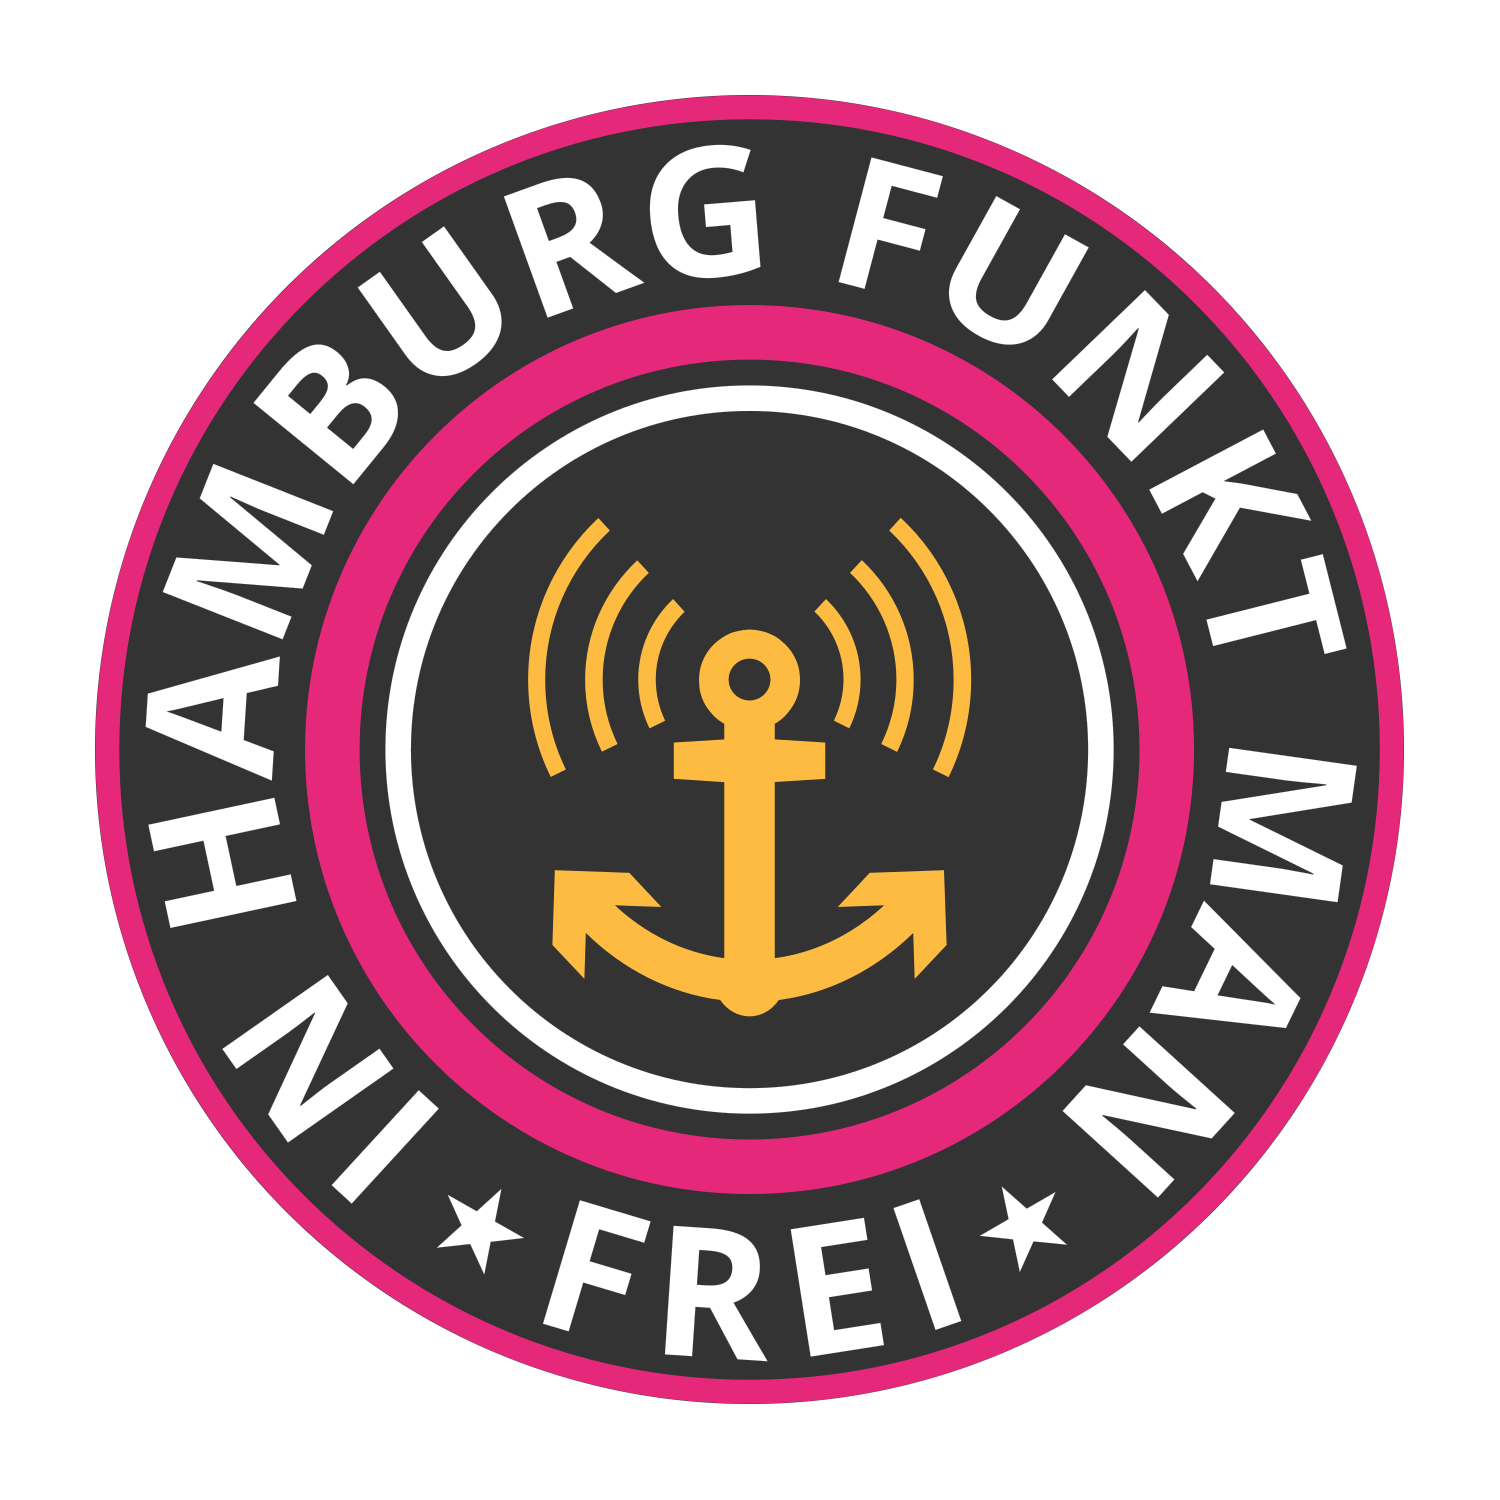
\includegraphics[width=65mm]{in-hamburg-funkt-man-frei.png}
\end{center}
\vspace{3em}
\begin{center}

\includegraphics[width=40mm]{qr.png}\\
\footnotesize https://t1p.de/0nzq\\Dieser Flyer als PDF.
\end{center}
\vfill
\section{Kontakt}
\begin{tabular}{ll}
WWW & \href{https://hamburg.freifunk.net}{https://hamburg.freifunk.net}\\
E-Mail & \href{mailto:kontakt@hamburg.freifunk.net}{kontakt@hamburg.freifunk.net}\\
        \\
Treffen & 14-tägig Montags, online\\
	& \href{https://hamburg.freifunk.net/kalender}{\small https://hamburg.freifunk.net/kalender}
\end{tabular}

\end{document}
